\chapter{APPLICATION DOMAINS}
\thispagestyle{plain}

\label{Domains}


Four target domains are used to demonstrate \fw in action, which show the effectiveness of \fw in a variety of different types of situations.
In Chapter \ref{Results}: Results, experiments are performed on each of these ABMs to evaluate \fw.
No modifications to \fw have to be performed to have \fw compatible with these domains, which shows that \fw is domain independent.
In each of the domains enumerated in this chapter, I give a brief overview of what the ABM represents, what configuration parameters are available, and what system-level properties I have defined.

\section{NetLogo Fires}\label{sec:Fires}

\begin{figure}[ht]
\centering
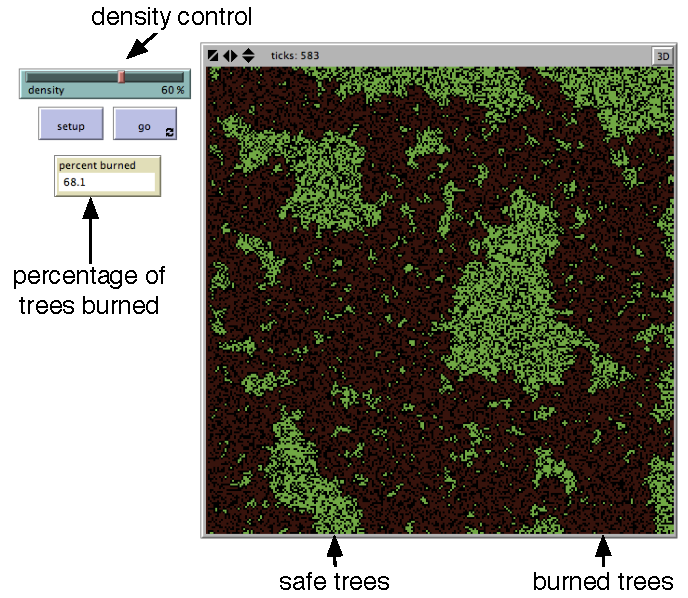
\includegraphics[scale=1]{images/fires_ui.pdf}
\caption{Screen capture of the Fires NetLogo ABM.}
\label{fig:firesui}
\end{figure}

The NetLogo Fires ABM is the simplest ABM tested in this dissertation.
In this ABM, trees are distributed throughout a $250 \times 250$ grid world.
A fire is started in the left column, in which all trees in this column burn.
Each burning tree then burns its adjacent trees (up, down, left, and right).
This process continues until no more trees are adjacent to burning trees.

The configuration space is one-dimensional and the system-level property space is one dimensional.
The configuration parameter for this domain is the density $\rho$ of the forest, which in our experiments I range from 45 \% to 75\%.
What this parameter does is change the probability that a grid point contains a tree.
During the initialization step, each grid point has a tree placed with probability $\rho$.
The system-level property is the percentage of trees burned down, which is measured by diving the number of trees that were burned by the total number of trees in the system.


The Fires ABM is particularly interesting because it exhibits a threshold effect.
There is a sharp transition from small amounts of the forest burning down and the entire forest burning down when the forest density increases past 58\%.
The behavior space is not linear and exhibits high variance around 58\%, making this ABM moderately challenging, regardless of it only having one configuration parameter.

%%%%%%%%%%%%%%%%%%%%%%%%%%%%%%%

 \section{NetLogo Flocking}

The NetLogo Flocking ABM is a classic agent-based model based on rules devised by Reynolds \cite{reynolds1987}.
As in the the original work, the flocking emergent behavior results from the summation of the following forces:
\begin{itemize}
	\item \textit{avoidance} -- repels agents that are too close to one another,
	\item \textit{center} -- attract agents towards the center of the flock,
	\item \textit{align} -- steer towards the average heading.
\end{itemize}

\begin{figure}[ht]
\centering
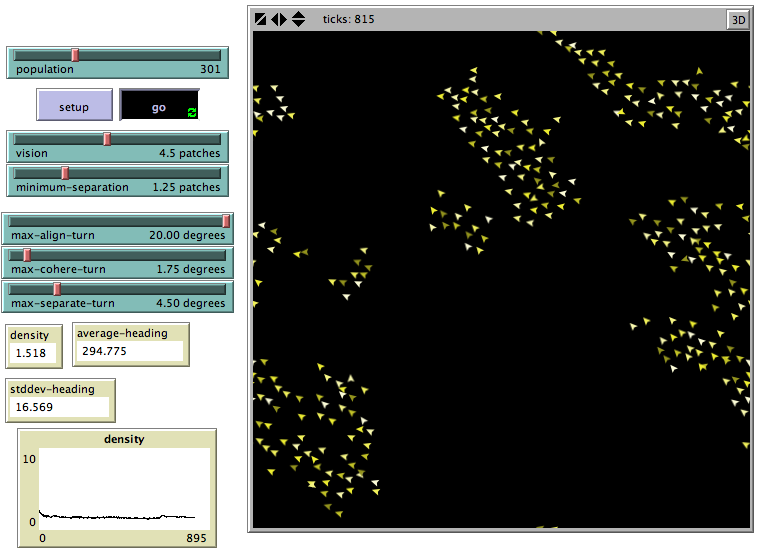
\includegraphics[scale=.333333]{images/flocking_ss.png}
\caption{Screen capture of the NetLogo Flocking ABM.}
\label{fig:flockingss}
\end{figure}

The NetLogo implementation of flocking follows the original definition closely.
There are six configuration parameters, as seen in Figure \ref{fig:flockingss}, however, only three are used:
\begin{itemize}
\item \textit{max-align-turn} -- the maximum amount of degrees an agent will turn to align heading with its neighbors,
\item \textit{max-cohere-turn} -- the maximum amount of degrees an agent will turn towards the center of the flock,
\item \textit{max-separate-turn} -- the maximum amount of degrees an agent will turn away if another agent is within \textit{minimum-separation}.
\end{itemize}
The other three configuration parameters available in the user interface (\textit{population}, \textit{vision}, and \textit{minimum-separation} are excluded because they do not affect the system-level properties as directly as the three outlined above.
The values for these parameters are kept constant throughout the experimentation performed for this thesis.

Two system-level properties are analyzed for this system:
\begin{itemize}
\item \textit{spread} -- measures how spread out the agents are.

This metric is calculated as the average distance from each agent to its nearest neighbor.
This calculation is an approximation to the true density, as it does not directly measure agents per patch.
Approximating is necessary because determining the area that an individual flock covers is not trivial and sometimes subjective.
In addition, a single instance could have several individual flocks, making this computation even more obscure.
The distance to the average neighbor captures the information that density conveys: as the distance increases, the agents are more spread out, and thus less dense.

\begin{figure}[ht]
\centering
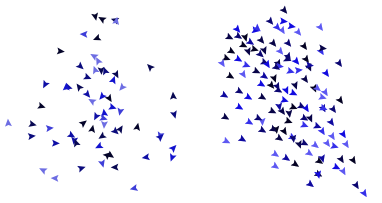
\includegraphics[scale=1]{images/swarmVSflock.png}
\caption{A swarming boid system (left) and a flocking boid system (right).}
\label{fig:swarmVSflock}
\end{figure}

\item \textit{stddev-heading} -- measures the standard deviation of the agent headings.

This metric is used to determine how much the agents in the ABM agree on the direction they are heading.
Configurations with agents that flock smoothly in one direction typically have a very low \textit{stddev-heading} value.
Meanwhile, more chaotic configurations will have a relatively high \textit{stddev-heading} value.
This contrast is illustrated in Figure \ref{fig:swarmVSflock}.

\end{itemize}

The Flocking ABM has the role that it is less challenging than Wolf Sheep Predation, but more complex than Fires.
The system-level properties change in a more monotonic and predictable manner than the other domains, but still remains sufficiently complex.
The behaviors are not linear and the configuration space is three-dimensional, making this problem still nontrivial. 

%%%%%%%%%%%%%%%%%%%%%%%%%%%%%



 \section{NetLogo Traffic Basic}

config: number-of-cars, acceleration, deceleration

slp: average max speed, average min speed, frequency of traffic jam






%%%%%%%%%%%%%%%%%%%%%%%5
 \section{NetLogo Wolf Sheep Predation}
The NetLogo Wolf Sheep Predation ABM has been the running example throughout this dissertation.
In this ABM, there are three major entities: wolves, sheep and grass.
Wolves eat sheep, sheep eat wolves and sheep eat grass.
The grass naturally regrows, meanwhile wolves and sheep occasionally reproduce.
Every time step sheep and wolves lose some energy and die naturally if their energy reaches zero.
A screen capture of the Wolf Sheep Predation ABM in NetLogo is shown in Figure \ref{fig:wolfsheepss}.
The configuration controls are in the top left, the monitors are in the bottom left and the visualization of the domain is on the right.

\begin{figure}[ht]
\centering
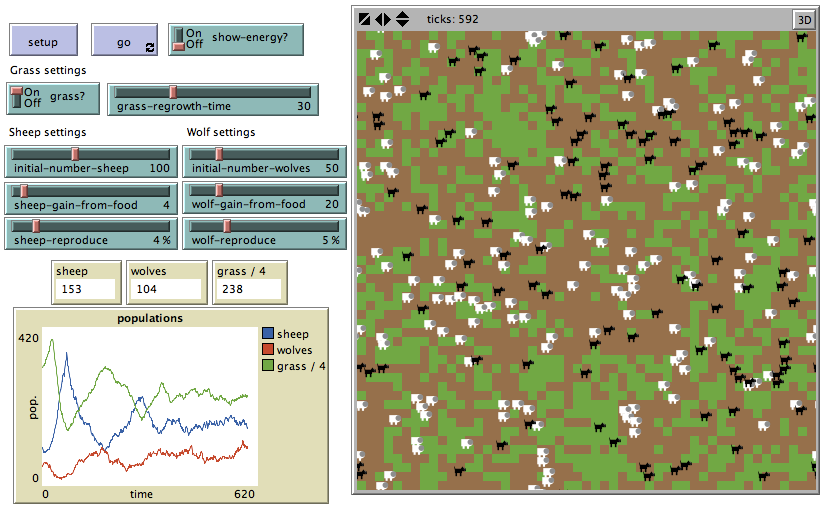
\includegraphics[scale=.4]{images/wolfsheep_ss.png}
\caption{Screen capture of the Wolf Sheep Predation ABM.}
\label{fig:wolfsheepss}
\end{figure}

The populations of a running Wolf Sheep Predation system are constantly changing.
Therefore, measuring properties is not as straightforward as in the Fires ABM.
Changes in populations can range from small oscillations to high magnitude oscillations in numbers, depending on the configuration parameters.
Quantitatively capturing these properties is challenging, but is possible with \fw.
A plot of a relatively normal (not too stable and not too high-magnitude) population is shown in Figure \ref{fig:wsp_norm}.

\begin{figure}[ht]
\centering
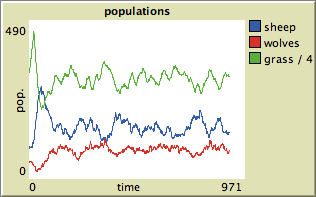
\includegraphics[scale=.666667]{images/wolfsheep/wolfsheep_normal.png}
\caption{Plot of a stable populations in a Wolf Sheep Predation system.}
\label{fig:wsp_norm}
\end{figure}


\begin{figure}[ht]
\centering
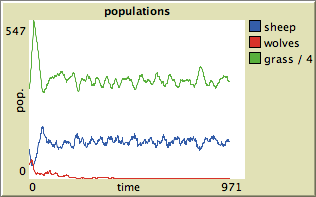
\includegraphics[scale=.666667]{images/wolfsheep/sheepfood_low.png}
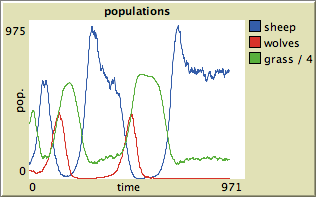
\includegraphics[scale=.666667]{images/wolfsheep/sheepfood_high.png}
\caption{Plot of a Wolf Sheep Predation run with low (left) and high (right) \textit{sheep-gain-form-food}.}
\label{fig:wsp_sheepfood}
\end{figure}


\begin{figure}[ht]
\centering
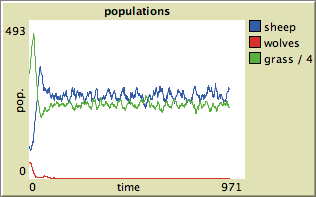
\includegraphics[scale=.666667]{images/wolfsheep/wolffood_low.png}
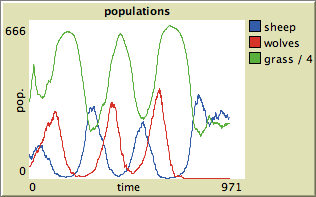
\includegraphics[scale=.666667]{images/wolfsheep/wolffood_high.png}
\caption{Plot of a Wolf Sheep Predation run with low (left) and high (right) \textit{wolf-gain-form-food}.}
\label{fig:wsp_wolffood}
\end{figure}


\begin{figure}[ht]
\centering
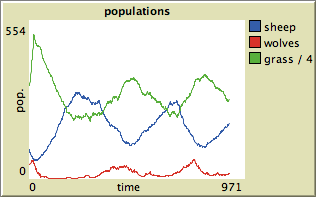
\includegraphics[scale=.666667]{images/wolfsheep/sheepsex_low.png}
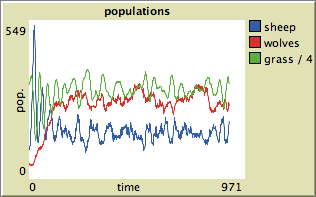
\includegraphics[scale=.666667]{images/wolfsheep/sheepsex_high.png}
\caption{Plot of a Wolf Sheep Predation run with low (left) and high (right) \textit{sheep-reproduce}.}
\label{fig:wsp_sheepsex}
\end{figure}


\begin{figure}[ht]
\centering
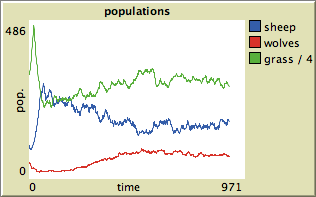
\includegraphics[scale=.666667]{images/wolfsheep/wolfsex_low.png}
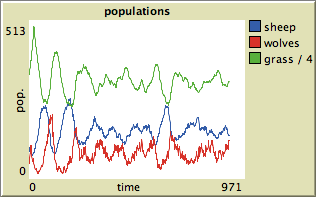
\includegraphics[scale=.666667]{images/wolfsheep/wolfsex_high.png}
\caption{Plot of a Wolf Sheep Predation run with low (left) and high (right) \textit{wolf-reproduce}.}
\label{fig:wsp_wolfsex}
\end{figure}


The configuration space is five-dimensional, making this domain nontrivial to analyze.
The configuration parameters, along with some general observations, are as follows:
\begin{itemize}
   \item \textit{sheep-gain-from-food} -- the amount of energy sheep gain from eating grass.
This parameter has interesting effects on the system.
The effect of changing this parameter from the stable norm is shown in Figure \ref{fig:wsp_sheepfood}.

At lower values, the population of the sheep has difficulty not going extinct.
This almost always results in the wolf population going extinct.

At higher values, sheep live longer and quickly become overpopulated, which causes the grass to become a scarce resource.
With little grass left, the sheep begin to die off.
Once enough sheep have died off, the grass begins to regrow and the sheep begin to reproduce.
This results in sharp increases and decreases in sheep population as the sheep population oscillates between overpopulated and underpopulated.
When the oscillations are of high enough magnitude, the wolves have a high chance of becoming extinct while the sheep population is very low.


   \item \textit{wolf-gain-from-food} -- the amount of energy wolves gain from eating a sheep.
This parameter affects the system in a similar way as \textit{sheep-gain-from-food}.
Lower values cause the wolves to go extinct, while higher values cause more drastic oscillations in wolf and sheep populations.
The effect of changing this parameter from the stable norm is  shown in Figure \ref{fig:wsp_wolffood}.

   \item \textit{sheep-reproduce} -- the percent chance that a sheep will reproduce, per time step.
This parameter has the interesting property that when it is increased, the wolf population increases, but the sheep population remains relatively constant.
When \textit{sheep-reproduce} is too low, the sheep population has difficulties sustaining its numbers, which causes the wolf population to be very low.
The effect of changing this parameter from the stable norm is  shown in Figure \ref{fig:wsp_sheepsex}.

   \item \textit{wolf-reproduce} -- the percent chance that a wolf will reproduce, per time step.
This parameter has relatively little effect on the system, in comparison to the other parameters.
The populations oscillate more when the reproduction rate is higher and more stable with it lower.
The effect of changing this parameter from the stable norm is  shown in Figure \ref{fig:wsp_wolfsex}.

   \item \textit{grass-regrowth-time} -- the amount of time steps a patch of grass takes to regrow.
This is perhaps the strangest behaving configuration parameter.
At higher values, not enough grass grows to sustain a large sheep population, which causes the wolves to go extinct.
At lower values, sheep rarely every die, until they become overpopulated and eat all the grass.
At this point, there is a mass extinction, which causes the wolves to typically go extinct.
In behavior, this parameter is similar to that of \textit{sheep-gain-from-food}.

\end{itemize}
Each of these parameters individually affect the system state.
Even more diverse behaviors can be observed by adjusting several parameters at once.

Several system-level properties have been developed for this domain.
To sample many of these properties and to provide more consistent results, each random configuration is sampled a number of times and averaged.
\begin{itemize}
\item \textit{sheep-extinct?} and \textit{wolves-extinct?} -- the probability that the sheep and wolf populations will reach zero, respectively.

The probability of sheep and wolf extinction is measured by sampling the same configuration numerous times and calculating the percentage of instances they went extinct.
Most often with a specific configuration, the sheep or wolves always go extinct or always do not go extinct.
However, there are borderline configurations in which the sheep or wolves will go extinct while the system is stabilizing into a rhythm.
This metric is useful in distinguishing between these three situations.
Wolves will always go extinct if there are no sheep, but sheep can exist without wolves.
Therefore, the value of \textit{wolves-extinct} is always higher than \textit{sheep-extinct?}.

\item \textit{sheep-average} and \textit{wolf-average} -- the average sheep and wolves given they did not go extinct, respectively.

The average sheep and wolf populations are calculated by averaging the populations at every time step in instances in which they did not go extinct.
Not including extinct populations in the average is important because these instances will introduce significant amounts of bias.
This metric describes how large the population can expected to be.
Along with \textit{sheep-variance} and \textit{wolf-variance}, the averages describes the nature of the population and how it changes.

\item \textit{sheep-variance} and \textit{wolf-variance} -- the variance of the sheep and wolf population over the course of a run.

The variance is calculated with the same data as the average.
This metric describes how much the population changes from time step to time step, since the population is typically rhythmically changing.

\end{itemize}

The Wolf Sheep Predation ABM is interesting because its behaviors are not linear and are not monotonic.
That is, as many of the configuration parameters increase, the resulting system-level behavior does not change in a linear manner.
This property of the behavior space makes many of the system-level properties difficult to predict.
In addition, there are five configuration parameters, which makes the configuration space five-dimensional.
The system-level property space is up to six dimensions.
Handling dimensionality up to eleven is a challenging task for any approach that is attempting to analyze system-level behavior.



